\section{Execution-conditioned planning}
\label{sec:method}
Our approach has two parts (\cref{fig:method}). Offline, interaction-biased data collection enriches the experience from which dynamics are learned. Online, ECP monitors execution and, once it detects a stall, modifies the next planning objective through a stagnation memory and a temporary goal reweighting that persist across replans.
\begin{figure*}[t]
\centering
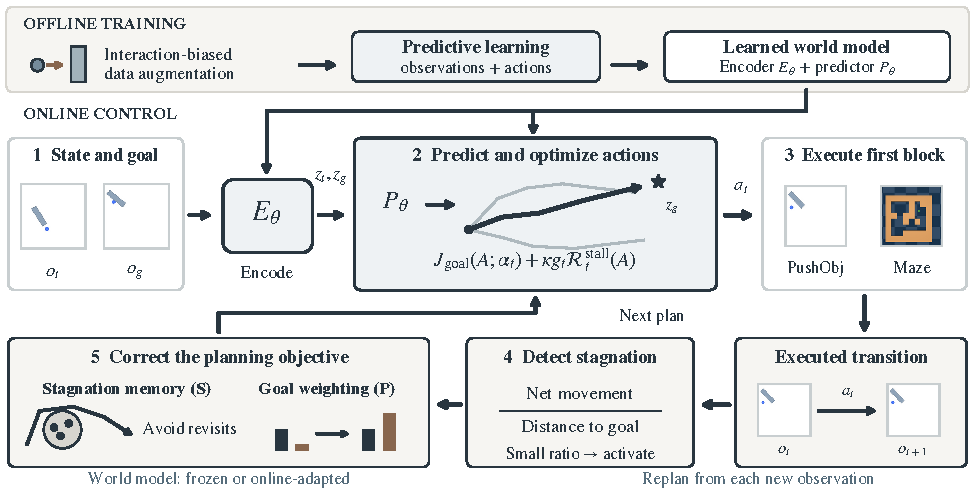
\includegraphics[width=\textwidth]{figures/fig2_method.pdf}
\caption{\textbf{ECP connects execution feedback to planning.} Offline actions combine contact bias with Gaussian noise before collection. Step 3 illustrates PushObj, Maze, shifted PushT, and Rope execution. Step 4 detects small net movement relative to goal distance. Step 5 retains stagnation memory ($S$) and boosts goal weighting ($P$) for three calls, renewed by new triggers. The timeline highlights sustained correction inspired by ACT. Model parameters may remain fixed or adapt online.}
\label{fig:method}
\end{figure*}

\subsection{Latent planning and the ECP objective}
At planning step $t$, the agent receives an observation $o_t=(x_t,p_t)$, consisting of an image $x_t$ and proprioception $p_t$, together with a goal observation $o_g$. An encoder $E_\theta$ maps them to latent states $z_t=(z_t^v,z_t^p)$ and $z_g$, whose visual and proprioceptive parts have dimensions $d_v$ and $d_p$. Given candidate action blocks $A=(a_1,\ldots,a_H)$ over a horizon $H$, an action-conditioned predictor $P_\theta$ produces future states $\hat z_{t,h}(A)$, $h=1,\ldots,H$. Model predictive control optimizes $A$, executes its first block, and replans from the resulting observation.

Planning quality is measured by a distance that balances the two branches of the latent state,
\begin{equation}
 D_\alpha(z,z')=
 \frac{\norm{z^v-z'^v}^2}{d_v}
 +\alpha\frac{\norm{z^p-z'^p}^2}{d_p},
 \label{eq:metric}
\end{equation}
where $\norm{\cdot}$ is the Euclidean norm and $\alpha\geq0$ weights proprioception. The planner's \emph{native} objective $J_{\rm goal}(A;\alpha)$ aggregates this distance to the goal along the rollout, at the terminal frame or over all frames depending on the underlying planner. Since $J_{\rm goal}$ depends only on the current observation and the goal, planning calls made from the same state are indistinguishable, whatever happened between them. ECP lets the objective depend on the episode instead:
\begin{equation}
 A_t^*=\argmin_A\left\{
 J_{\rm goal}(A;\alpha_t)
 +\kappa g_t\mathcal R_t^{\rm stall}(A)\right\}.
 \label{eq:objective}
\end{equation}
Here $\mathcal R_t^{\rm stall}$ is a stagnation regularizer built from an episode memory $\mathcal M_t$, $\kappa$ is its strength, $g_t\in\{0,1\}$ gates its activation, and $\alpha_t$ is a goal weight that can be raised temporarily above its base value $\alpha_0$. Until a stall is detected, the memory is empty and $\alpha_t=\alpha_0$, so \cref{eq:objective} coincides exactly with native planning. ECP thus changes only the action objective: the encoder, predictor, and optimizer are untouched, and $\theta$ may stay fixed or be updated online.

\subsection{Detecting stagnation from execution}
\label{sec:trigger}
A stall detector must separate lack of progress from lack of motion, since a stalled controller can execute large actions and still end where it began. We therefore compare the \emph{net} latent displacement over a window of $W$ observation-feedback steps with the distance that remains to the goal:
\begin{equation}
 r_t=\sqrt{\frac{D_{\alpha_0}(z_t,z_{t-W})}
 {\max\{D_{\alpha_0}(z_t,z_g),\epsilon\}}},
 \label{eq:rate}
\end{equation}
where $z_{t-W}$ is the state $W$ feedback steps earlier and $\epsilon$ is a numerical floor. The ratio compares net motion with remaining goal distance: small $r_t$ indicates little movement relative to the task still ahead. It is invariant to uniform latent rescaling when the numerical floor is inactive. We map it to a continuous stall weight,
\begin{equation}
 w_t=\operatorname{clip}_{[0,1]}\!\left(
 \frac{\gamma_{\rm hi}-r_t}{\gamma_{\rm hi}-\gamma_{\rm lo}}\right),
 \label{eq:weight}
\end{equation}
which equals one below $\gamma_{\rm lo}$, decreases linearly between the thresholds, and is zero above $\gamma_{\rm hi}$. Whenever $w_t>0$, the pair $(o_t,w_t)$ is appended to the episode memory $\mathcal M_t$. Because current, past, and goal observations are all encoded by the current encoder, the detector stays consistent under online adaptation.

\subsection{Stagnation memory}
\label{sec:memory}
The memory turns detected stalls into a cost that discourages predicted trajectories from re-entering stalled neighborhoods, while leaving the goal and unrelated regions of the latent space unaffected. Before each planning call, every stored observation is re-encoded as a memory state $m_j$, where $j$ indexes the entries of $\mathcal M_t$ and $w_j$ is the recorded stall weight. Let $d_j=D_{\alpha_0}(m_j,z_g)$ be its squared goal distance. The penalty amplitude $s_j$ and squared support radius $\rho_j$ are
\begin{equation}
 s_j=\frac{d_j}{H+1},\qquad
 \rho_j=\max\{\beta d_j,\epsilon\}.
 \label{eq:memoryscale}
\end{equation}
Here $\beta\in(0,1)$ sets the neighborhood size, and $1/(H+1)$ matches the all-frame goal objective's scale. A compact-support kernel penalizes predicted states near the memory,
\begin{equation}
 K_j(z)=\left[1-\frac{D_{\alpha_0}(z,m_j)}{\rho_j}\right]_+^2,
 \label{eq:kernel}
\end{equation}
where $[u]_+=\max(u,0)$. The kernel is one at $m_j$ and zero when $D_{\alpha_0}(z,m_j)\geq\rho_j$. Summing over memories and the horizon gives
\begin{equation}
 \mathcal R_t^{\rm stall}(A)
 =\sum_{h=1}^{H}\pi_h
 \sum_{j\in\mathcal M_t}w_js_jK_j(\hat z_{t,h}(A)),
 \label{eq:penalty}
\end{equation}
in which the normalized weights $\pi_h=2^h/\sum_{k=1}^{H}2^k$ emphasize later frames and thus favor plans that end outside a stalled neighborhood. Memories persist throughout the episode. The fixed-strength Rope variant assigns unit weight to every triggered memory instead of retaining its severity $w_j$.

Tying the amplitude and the radius to the goal distance gives the regularizer two useful properties, derived in \cref{sec:properties}. It never penalizes the goal: because $\beta<1$, the support of each kernel is strictly smaller than the distance from its memory to the goal, so, above the numerical floor $\epsilon$, the goal lies outside every support. It is also smooth and local: the penalty and its first derivative vanish at the support boundary and beyond, so plans that stay away from stalled neighborhoods are optimized exactly as before.

\subsection{Temporary goal reweighting}
\label{sec:weighting}
Memory tells the planner where not to return; it does not tell it what to finish. A controller can stall with one goal component nearly satisfied and another still open: in PushObj, once the object is nearly aligned, the remaining error lies in the pusher position, which the proprioceptive branch of \cref{eq:metric} measures directly. When a stall is detected and the correction gate is open, ECP therefore raises the proprioceptive weight to $\alpha_t=b\,\alpha_0$, with $b>1$, for a fixed number of planning calls. A new trigger renews this interval; otherwise the weight returns to $\alpha_0$. Because the boost is conditional and temporary, the native objective governs planning whenever execution is progressing.

\subsection{Coordinating correction with online adaptation}
\label{sec:gate}
In its trigger-only mode, ECP sets $g_t=1$ throughout, and the empty memory guarantees native behavior before the first trigger. When the world model adapts online, however, a stall may resolve through continued learning, and the objective needs to change only once learning has plateaued. A gated mode detects this from the prediction error. Let $\ell_t$ be the mean squared prediction error on the newest executed transition, measured before its model update, and $\bar\ell_t$ its short running mean. The relative improvement over a separation of $W_g$ steps is
\begin{equation}
 q_t=\frac{\bar\ell_{t-W_g}-\bar\ell_t}
 {\max\{\bar\ell_{t-W_g},\epsilon\}}.
 \label{eq:gate}
\end{equation}
Positive $q_t$ means the prediction loss has fallen; zero or negative values indicate a plateau or increase. Starting from $g_t=0$, the gate opens when the controller is stalled ($w_t>0$) and improvement falls below a minimum $\tau_g$ ($q_t<\tau_g$), and remains open thereafter. Stalled observations are recorded while the gate is closed, so the memory is available as soon as correction begins.

\subsection{Interaction-biased data augmentation}
\label{sec:data}
ECP corrects stalls as they occur; the training data influences how often they occur in the first place, since a world model can only predict the interactions it has seen. Following AdaJEPA's contact-biased collection~\cite{wang2026adajepa} and inspired by the noise injection of DART~\cite{laskey2017dart}, we add an object-directed offset and Gaussian noise to each source action $u_i$ at control step $i$, giving $u_i+b_c\operatorname{unit}(c_i-p_i)+\sigma_c\eta_i$. Here $c_i,p_i\in\R^2$ are the object center and pusher position, $\operatorname{unit}(\cdot)$ normalizes a nonzero vector, $\eta_i\sim\mathcal N(0,I_2)$, and $b_c$ and $\sigma_c$ set the bias and noise scales. The perturbed actions are executed in the simulator, and every retained trajectory contains contact. The training objective, latent prediction with trajectory straightening~\cite{wang2026straightening}, is left unchanged; \cref{sec:implementation} gives the complete recipe.
